\begin{minipage}[b]{0.33\linewidth}
\begin{lrbox}{\mybox}%
\begin{lstlisting}[basicstyle=\ttfamily\tiny]
* = $0801
;-------------------------
; Start program at InitializeProgram (SYS 2064)
; SYS 2064 ($0810)
;-------------------------
 .BYTE $0B,$08          
 .BYTE $C1,$07          
 .BYTE $9E              
 .BYTE $32,$30,$36,$34 
 .BYTE $00              
 .BYTE $00,$00          
 .BYTE $F9,$02,$F9      

;----------------------
; LaunchPsychedelia
;----------------------
LaunchPsychedelia
 JSR InitializeScreenLinePtrArray
 JSR ClearScreen
 JSR SetUpInterrupts
 SEI 
 JSR InitializePsychedelia
 JSR SetUpBackgroundPainting
 JSR InitializeColorIndexArray
 JSR InitializeStatusDisplayText
 JSR UpdateCurrentSettingsDisplay
 CLI 
PsychedeliaLoop   
 JSR MaybeUpdateFromBuffersAndPaint
 JSR CheckKeyboardInput
 JMP PsychedeliaLoop

a40D7   .BYTE $03
a4142   .BYTE $01
;--------------------------
; SetUpInterrupts
;--------------------------
SetUpInterrupts   
 SEI 
 LDA #$7F
 STA $DC0D    ;CIA1: CIA Interrupt Control Register
 LDA #<TitleScreenInterruptHandler
 STA $0314    ;IRQ
 LDA #>TitleScreenInterruptHandler
 STA $0315    ;IRQ
 LDA #$00
 STA currentRasterArrayIndex
 JSR UpdateRasterPosition
 JSR InitializeRasterJumpTablePtrArray

 LDA #$01
 STA $D01A    ;VIC Interrupt Mask Register (IMR)
 RTS 

;--------------------------
; UpdateRasterPosition
;--------------------------
UpdateRasterPosition   
 LDA $D011    ;VIC Control Register 1
 AND #$7F
 STA $D011    ;VIC Control Register 1
 LDX currentRasterArrayIndex
 LDA rasterPositionArray,X
 CMP #$FF
 BNE b4224

 LDA #$00
 STA currentRasterArrayIndex
 LDA rasterPositionArray
b4224   STA $D012    ;Raster Position
 LDA #$01
 STA $D019    ;VIC Interrupt Request Register (IRR)
 RTS 

rasterJumpTableLoPtr2=*+$01
rasterJumpTableLoPtr3=*+$02
rasterJumpTableLoPtrArray 
 .BYTE $55,$55
 .BYTE $22,$22,$22,$22,$46,$46,$46,$46
 .BYTE $46,$46
rasterJumpTableHiPtr2=*+$01
rasterJumpTableHiPtr3=*+$02
rasterJumpTableHiPtrArray 
 .BYTE $C0,$C0
 .BYTE $C3,$C3,$C3,$C3,$42,$42,$42,$42
 .BYTE $42,$42
rasterPositionArray       
 .BYTE $E0,$FF,$C0,$FF,$A0,$C0,$FF

;--------------------------
; InitializeRasterJumpTablePtrArray
;--------------------------
InitializeRasterJumpTablePtrArray   
 LDX #$00
b4574
 LDA #$46
 STA rasterJumpTableLoPtrArray,X
 LDA #$42
 STA rasterJumpTableHiPtrArray,X
 INX 
 CPX #$0C
 BNE b4574
 RTS 

\end{lstlisting}
\end{lrbox}%
\scalebox{0.8}{\usebox{\mybox}}
\end{minipage}
\hspace{0.5cm}
\begin{minipage}[b]{0.33\linewidth}
\begin{lrbox}{\mybox}%
\begin{lstlisting}[basicstyle=\ttfamily\tiny]
;--------------------------
; TitleScreenInterruptHandler
;--------------------------
TitleScreenInterruptHandler
 LDA $D019    ;VIC Interrupt
 AND #$01
 BNE b4237
 JMP $EA31
 ; Returns

 ; After a delay calculated from the 
 ; IRQ switch to the Zarjas poster
 ; and back again.
b4237
 LDX currentRasterArrayIndex
 LDA rasterJumpTableLoPtrArray,X
 STA a08

 LDA rasterJumpTableHiPtrArray,X
 STA a09

 JMP ($0008)
 ;Returns

;--------------------------
; ClearScreen
;--------------------------
ClearScreen   
 LDX #$00
_Loop
 LDA #SPACE
 STA SCREEN_RAM,X
 STA SCREEN_RAM + $0100,X
 STA SCREEN_RAM + $0200,X
 STA SCREEN_RAM + $0300,X

 LDA #WHITE
 STA COLOR_RAM + $02F0,X
 DEX 
 BNE _Loop
 RTS 

;--------------------------
; InitializeScreenLinePtrArray
;--------------------------
InitializeScreenLinePtrArray   
 LDA #>SCREEN_RAM
 STA screenLinesHiPtr
 LDA #<SCREEN_RAM
 STA screenLinesLoPtr

 LDX #$00
b414D
 LDA screenLinesLoPtr
 STA screenLinesLoPtrArray,X
 LDA screenLinesHiPtr
 STA screenLinesHiPtrArray,X
 LDA screenLinesLoPtr
 CLC 
 ADC #NUM_COLS
 STA screenLinesLoPtr

 LDA screenLinesHiPtr
 ADC #$00
 STA screenLinesHiPtr
 INX 
 CPX #NUM_ROWS + 2
 BNE b414D
 RTS 

;--------------------------
; GetCurrentCharAddress
;--------------------------
GetCurrentCharAddress   
 LDX currentCharYPos
 LDY currentCharXPos

 LDA screenLinesLoPtrArray,X
 STA screenLinesLoPtr

 LDA screenLinesHiPtrArray,X
 STA screenLinesHiPtr
 RTS 

;--------------------------
; WriteCurrentCharToScreen
;--------------------------
WriteCurrentCharToScreen   
 JSR GetCurrentCharAddress

 LDA currentChar
 STA (screenLinesLoPtr),Y

 LDA screenLinesHiPtr
 PHA 

 ; Update color of character
 CLC 
 ADC #OFFSET_TO_COLOR_RAM
 STA screenLinesHiPtr

 LDA defaultColorValue
 STA (screenLinesLoPtr),Y

 PLA 
 STA screenLinesHiPtr
 RTS 


\end{lstlisting}
\end{lrbox}%
\scalebox{0.8}{\usebox{\mybox}}
\end{minipage}
\hspace{0.5cm}
\begin{minipage}[b]{0.33\linewidth}
\begin{lrbox}{\mybox}%
\begin{lstlisting}[basicstyle=\ttfamily\tiny]
;----------------------
; InitializePsychedelia
;----------------------
InitializePsychedelia   
 LDX #$00
_Loop
 LDA #SPACE
 STA SCREEN_RAM,X
 DEX 
 BNE _Loop

 LDA $D016    ;VIC Control
 AND #$F0
 ORA #$08
 STA $D016    ;VIC Control

 LDA #$18
 STA $D018    ;VIC Memory

 LDA #BLACK
 STA $D020    ;Border 
 STA $D021    ;Background
 STA $D400    ;Voice 1

 LDA #$04
 STA $D407    ;Voice 2

 LDA #$08
 STA $D40E    ;Voice 3

 LDA #TOP_Y_POSITION - 7
 STA currentCharYPos

 LDA #$63
 STA currentChar

 LDA currentColorValue
 STA defaultColorValue

SetUpScreenLoop   
 LDA #$00
 STA currentCharXPos

InnerLoop  
 JSR WriteCurrentCharToScreen

 LDA currentCharYPos
 PHA 
 SEC 
 SBC #TOP_Y_POSITION - 7
 STA currentCharYPos

 LDA currentChar
 PHA 
 CLC 
 CLC 
 ADC #$5D
 STA currentChar

 JSR WriteCurrentCharToScreen

 PLA 
 STA currentChar

 PLA 
 STA currentCharYPos

 INC currentCharXPos

 LDA currentCharXPos
 CMP #NUM_COLS
 BNE InnerLoop

 INC currentChar
 INC currentCharYPos
 LDA currentCharYPos
 CMP #TOP_Y_POSITION + 1
 BNE SetUpScreenLoop

SetUpSpritesAndVoiceRegisters
 LDA $D011 ;VIC Control Register 1
 AND #$F8
 ORA #$03
 STA $D011 ;VIC Control Register 1

 LDA #$00
 STA $D015 ;Sprite display Enable
 STA a40D7
 STA a4142
 STA $D404 ;Voice 1: Control Register
 STA $D40B ;Voice 2: Control Register
 STA $D412 ;Voice 3: Control Register

DrawTwoMiddleLines
 LDX #$00
_Loop   
 LDA #$42
 STA SCREEN_RAM + (NUM_COLS * 8),X

 LDA currentColorValue
 STA COLOR_RAM + (NUM_COLS * 8),X

 INX 
 CPX #(2 * NUM_COLS)
 BNE _Loop
 RTS 
\end{lstlisting}
\end{lrbox}%
\scalebox{0.8}{\usebox{\mybox}}
\end{minipage}
\clearpage

\begin{definition}[Jeffrey Says]
\setlength{\intextsep}{0pt}%
\setlength{\columnsep}{3pt}%
\begin{wrapfigure}{l}{0.12\textwidth}

\includegraphics[width=\linewidth]{src/callout/psych.png} 
\end{wrapfigure}
\small
Well I was going to put a PAUSE mode in, but this is much better. When you need to, drop into SUB6 and relax. The timer stops and you can stay in the subgame until you've got your head together enough to play on. The controls are a subset of real PSYCHEDELIA, allowing S=symmetry change and C=cursor speed. You can also use F1 and SHIFT-F1 to change fore- and background colours.

\textbf{Design Notes:} Well it's more interesting than freezing the screen.
\end{definition}

The feel and appearance of this light synthesizer is familiar enough and as we shall see the overall structure of its internals have not radically changed from the
code we analysed in its predecessor. However closer inspection will reveal some subtle changes in the algorithm, some optimization and simplifications,
that mean this is not just a desultory lift-and-shift of previous work to fill a gap in a game in need of a pause mode.

Even a cursory glance at the screenshots below shows an overall change in the aesthetic, an attempt within the confines of the C64's limited capabilities to create
a less obviously pixellated appearance, an attempt create an impression of blur and flow:

\begin{figure}[H]
    \begin{adjustbox}{width=13cm,center}
    \frame{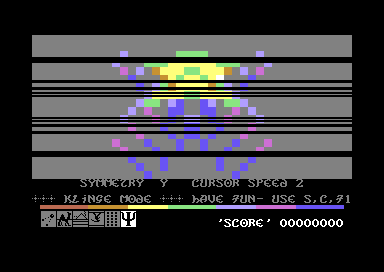
\includegraphics{src/batalyx_patterns/batalyx1.png}}%
      \hspace{0.2cm}
    \frame{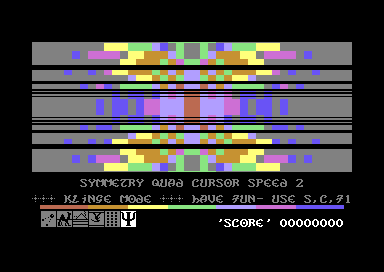
\includegraphics{src/batalyx_patterns/batalyx2.png}}%
    \end{adjustbox}
\caption{The Psychedelia sub-game in Batalyx. 'Y' symmetry on the left, and 'Quad' symmetry on the right.}
\end{figure}

Before we take a look at the core routines in detail, with a view to teasing out how they have evolved from their equivalents in Psychedelia, we should note how small
the code involved has remained. It takes up a total of just three and a half pages here and in those that follow. The only reason it is slightly larger than the
listing we reviewed in \hyperref[sec:listing_commentary]{\textcolor{blue}{'let's pretend we can read code'.}} is the overhead entailed in adding a scrolling receding
background. This effect is achieved with a neat conjunction of interrupt handlers, character set swapping, and a bit of brute force.

\clearpage
\begin{minipage}[b]{0.33\linewidth}
\begin{lrbox}{\mybox}%
\begin{lstlisting}[basicstyle=\ttfamily\tiny]
;----------------------
; SetUpBackgroundPainting
;----------------------
SetUpBackgroundPainting   
 LDX #$00
b78A4   
 LDA psyRasterPositionArray,X
 STA rasterPositionArray,X
 LDA psyRasterJumpTableLoPtrArray,X
 STA rasterJumpTableLoPtrArray,X
 LDA psyRasterJumpTableHiPtrArray,X
 STA rasterJumpTableHiPtrArray,X
 INX 
 CPX #$03
 BNE b78A4
 RTS 

psyRasterPositionArray       
 .BYTE $C0,$FF,$FF
psyRasterJumpTableLoPtrArray 
 .BYTE <PaintBackgroundColor,<PaintBackgroundColori
 .BYTE <PaintBackgroundColor
psyRasterJumpTableHiPtrArray 
 .BYTE >PaintBackgroundColor,>PaintBackgroundColor
 .BYTE >PaintBackgroundColor

;--------------------------
; IncrementAndUpdateRaster
;--------------------------
IncrementAndUpdateRaster
 INC currentRasterArrayIndex
 JSR UpdateRasterPosition
 PLA 
 TAY 
 PLA 
 TAX 
 PLA 
 RTI 

;----------------------
; PaintBackgroundColor
;----------------------
PaintBackgroundColor
 LDA currentBackgroundColor
 AND #$0F
 STA $D020    ;Border Color
 STA $D021    ;Background Color 0

 JSR UpdateBackgroundData
 JSR FetchBackgroundData
 JSR WriteLinesToScreen
 JSR $FF9F ;$FF9F - scan keyboard                    
 JMP IncrementAndUpdateRaster

currentColorValue .BYTE $0B
cursorXPosition   .BYTE $15
cursorYPosition   .BYTE $0B
colorValueToWrite .BYTE $01


screenRAMLoPtr = $23
screenRAMHiPtr = $24
;----------------------
; WriteValueToColorRAM
;----------------------
WriteValueToColorRAM   
 LDY cursorXPosition
 LDX cursorYPosition

 LDA screenLinesLoPtrArray,X
 STA screenRAMLoPtr

 LDA screenLinesHiPtrArray,X
 CLC 
 ADC #OFFSET_TO_COLOR_RAM
 STA screenRAMHiPtr

 LDA colorValueToWrite
 STA (screenRAMLoPtr),Y
 RTS 

;----------------------
; WriteLinesToScreen
;----------------------
WriteLinesToScreen   
 LDA currentColorValue
 STA colorValueToWrite

 JSR WriteValueToColorRAM
 JSR MaybeCheckJoystickInput

 LDA #WHITE
 STA colorValueToWrite

 JSR WriteValueToColorRAM
 RTS 

;----------------------
; MaybeCheckJoystickInput
;----------------------
MaybeCheckJoystickInput   
 DEC prevCursorSpeed
 BEQ CheckJoystickInput
 RTS 

prevCursorSpeed   .BYTE $02

\end{lstlisting}
\end{lrbox}%
\scalebox{0.8}{\usebox{\mybox}}
\end{minipage}
\hspace{0.5cm}
\begin{minipage}[b]{0.33\linewidth}
\begin{lrbox}{\mybox}%
\begin{lstlisting}[basicstyle=\ttfamily\tiny]
;----------------------
; CheckJoystickInput   
;----------------------
CheckJoystickInput   
 LDA cursorSpeed
 STA prevCursorSpeed
 ;CIA1: Data Port Register A
 LDA $DC00    
 STA lastJoystickInput

MaybeUpPressed
 AND #JOYSTICK_DOWN
 BEQ MaybeDownPressed

UpPressed
 DEC cursorYPosition
 LDA cursorYPosition
 CMP #BELOW_ZERO
 BNE MaybeDownPressed

 LDA #TOP_Y_POSITION
 STA cursorYPosition

MaybeDownPressed   
 LDA lastJoystickInput
 AND #JOYSTICK_UP
 BEQ MaybeLeftPressed

DownPressed
 INC cursorYPosition
 LDA cursorYPosition
 CMP #TOP_Y_POSITION+1
 BNE MaybeLeftPressed

 LDA #$00
 STA cursorYPosition

MaybeLeftPressed   
 LDA lastJoystickInput
 AND #JOYSTICK_RIGHT
 BEQ MaybeRightPressed

LeftPressed
 DEC cursorXPosition
 LDA cursorXPosition
 CMP #BELOW_ZERO
 BNE MaybeRightPressed

 LDA #NUM_COLS-1
 STA cursorXPosition

MaybeRightPressed   
 LDA lastJoystickInput
 AND #JOYSTICK_LEFT
 BEQ CheckFireButton

RightPressed
 INC cursorXPosition
 LDA cursorXPosition
 CMP #NUM_COLS
 BNE CheckFireButton

 LDA #$00
 STA cursorXPosition

CheckFireButton   
 JSR MaybeFirePressed
 RTS 

colorRAMLoPtr = $25
colorRAMHiPtr = $26
;----------------------
; PaintPixel
;----------------------
PaintPixel   
 LDX initialPixelYPosition
 LDY initialPixelXPosition
 LDA screenLinesLoPtrArray,X
 STA colorRAMLoPtr

 LDA screenLinesHiPtrArray,X
 CLC 
 ADC #OFFSET_TO_COLOR_RAM
 STA colorRAMHiPtr

 LDA (colorRAMLoPtr),Y
 AND #$0F
 CMP currentColorValue
 BEQ ActuallyPaintPixel

 TAX 
 LDA colorComparisonArray,X
 CMP lastColorValue
 BEQ ActuallyPaintPixel
 BPL ActuallyPaintPixel
 RTS 

ActuallyPaintPixel   
 LDA currentColor
 STA (colorRAMLoPtr),Y
 RTS 

colorComparisonArray   
 .BYTE ORANGE,ORANGE,WHITE
 .BYTE ORANGE,BLUE,PURPLE,YELLOW,CYAN
 .BYTE RED,ORANGE,ORANGE,ORANGE
 .BYTE ORANGE,ORANGE,GREEN,ORANGE
 .BYTE ORANGE
\end{lstlisting}
\end{lrbox}%
\scalebox{0.8}{\usebox{\mybox}}
\end{minipage}
\hspace{0.5cm}
\begin{minipage}[b]{0.33\linewidth}
\begin{lrbox}{\mybox}%
\begin{lstlisting}[basicstyle=\ttfamily\tiny]
lastColorValue        .BYTE $07
currentColor          .BYTE $0B
initialPixelYPosition .BYTE $0C
initialPixelXPosition .BYTE $0C

;----------------------
; PaintPixelForCurrentSymmetry
;----------------------
PaintPixelForCurrentSymmetry   
 LDA initialPixelYPosition
 AND #$80
 BEQ CanPaintPixelOnThisLine

CleanUpAndReturn   
 RTS 

CanPaintPixelOnThisLine   
 LDA initialPixelYPosition
 CMP #TOP_Y_POSITION+1
 BPL CleanUpAndReturn

 LDA initialPixelXPosition
 AND #$80
 BNE CleanUpAndReturn

 LDA initialPixelXPosition
 CMP #NUM_COLS
 BPL CleanUpAndReturn

 LDA currentColor
 TAX 

 LDA colorComparisonArray,X
 STA lastColorValue
 DEC lastColorValue

 JSR PaintPixel

 LDA currentSymmetrySettingForStep
 BNE HasSymmetry

ReturnFromSymmetry   
 RTS 

HasSymmetry   
 CMP #X_Y_SYMMETRY
 BEQ HasXYSymmetry

 CMP #X_AXIS_SYMMETRY
 BEQ HasXAxisSymmetry

 LDA #NUM_COLS-1
 SEC 
 SBC initialPixelXPosition
 STA initialPixelXPosition

 JSR PaintPixel

 LDA currentSymmetrySettingForStep
 CMP #Y_AXIS_SYMMETRY
 BEQ ReturnFromSymmetry

 LDA #TOP_Y_POSITION
 SEC 
 SBC initialPixelYPosition
 STA initialPixelYPosition

 JSR PaintPixel

 LDA #NUM_COLS-1
 SEC 
 SBC initialPixelXPosition
 STA initialPixelXPosition

 JMP PaintPixel

HasXYSymmetry   
 LDA #TOP_Y_POSITION
 SEC 
 SBC initialPixelYPosition
 STA initialPixelYPosition

 JMP PaintPixel

HasXAxisSymmetry   
 LDA #NUM_COLS-1
 SEC 
 SBC initialPixelXPosition
 STA initialPixelXPosition

 JMP HasXYSymmetry

currentSymmetrySettingForStep
.BYTE $01
presetColorValuesArray        
 .BYTE RED,ORANGE
 .BYTE YELLOW
 .BYTE GREEN,LTBLUE
 .BYTE PURPLE,BLUE
unusedVariable                
 .BYTE $0B
currentLineInPattern          
 .BYTE $07
currentPatternIndex           
 .BYTE $13
lastJoystickInput
 .BYTE $7F

\end{lstlisting}
\end{lrbox}%
\scalebox{0.8}{\usebox{\mybox}}
\end{minipage}
Before we take a look at the core routines in detail, with a view to teasing out how they have evolved from their equivalents in Psychedelia, we should note how small
the code involved has remained. It takes up a total of just three and a half pages here and in those that follow. The only reason it is slightly larger than the
listing we reviewed in \hyperref[sec:listing_commentary]{\textcolor{blue}{'let's pretend we can read code'.}} is the overhead entailed in adding a scrolling receding
background. This effect is achieved with a neat conjunction of interrupt handlers, character set swapping, and a bit of brute force.

\begin{minipage}[b]{0.33\linewidth}
\begin{lrbox}{\mybox}%
\begin{lstlisting}[basicstyle=\ttfamily\tiny]
;----------------------
; PaintStructureAtCurrentPosition
;----------------------
PaintStructureAtCurrentPosition   
 LDA #$00
 STA currentPatternIndex
 STA currentLineInPattern

 LDA currentPixelXPosition
 STA initialPixelXPosition

 LDA currentPixelYPosition
 STA initialPixelYPosition

 JSR PaintPixelForCurrentSymmetry

 LDA currentColorIndex
 BNE PixelPaintLoop
 RTS 

PixelPaintLoop   
 LDX currentPatternIndex
 LDA patternXPosArray,X
 CMP #$55
 BEQ MoveToNextLineInPattern

 CLC 
 ADC currentPixelXPosition
 STA initialPixelXPosition

 LDA patternYPosArray,X
 CLC 
 ADC currentPixelYPosition
 STA initialPixelYPosition

 JSR PaintPixelForCurrentSymmetry

 INC currentPatternIndex
 JMP PixelPaintLoop

MoveToNextLineInPattern   
 INC currentPatternIndex
 INC currentLineInPattern

 LDA currentLineInPattern
 CMP currentColorIndex
 BNE PixelPaintLoop
 RTS 

patternXPosArray             
 .BYTE $FF,$01,$55    ; 6              
 .BYTE $FE,$02,$55    ;            5   
 .BYTE $FD,$03,$55    ;   4            
 .BYTE $FC,$04,$55    ;          3     
 .BYTE $FB,$05,$55    ;     2          
 .BYTE $FA,$06,$55    ;        1       
 .BYTE $55,$55        ;                
patternYPosArray             ;      1         
 .BYTE $01,$FF,$55    ;         2      
 .BYTE $FE,$02,$55    ;    3           
 .BYTE $03,$FD,$55    ;           4    
 .BYTE $FC,$04,$55    ;  5             
 .BYTE $05,$FB,$55    ;             6 
 .BYTE $FA,$06,$55
 .BYTE $55,$55


currentColorIndex     .BYTE $07
currentPixelXPosition .BYTE $15
currentPixelYPosition .BYTE $06
sYmmetrySettingForStep
 .BYTE $01,$01,$01,$01,$01,$01,$01,$01
 .BYTE $01,$01,$01,$01,$01,$01,$01,$01
 .BYTE $01,$01,$01,$01,$01,$01,$01,$01
 .BYTE $01,$01,$01,$01,$01,$01,$01,$01
 .BYTE $01,$01,$01,$01,$01,$01,$01,$01
 .BYTE $01,$01,$01,$01,$01,$01,$01,$01
 .BYTE $01,$01,$01,$01,$01,$01,$01,$01
 .BYTE $01,$01,$01,$01,$01,$01,$01,$01

pixelXPositionArray   
 .BYTE $15,$15,$15,$15,$15,$15,$15,$15
 .BYTE $15,$15,$15,$15,$15,$15,$15,$15
 .BYTE $15,$15,$15,$15,$15,$15,$15,$15
 .BYTE $15,$15,$15,$15,$15,$15,$15,$15
 .BYTE $15,$15,$15,$15,$15,$15,$15,$15
 .BYTE $15,$15,$15,$15,$15,$14,$15,$16
 .BYTE $17,$18,$19,$1A,$1B,$1C,$1D,$1D
 .BYTE $1D,$1C,$1B,$1A,$19,$18,$17,$16

pixelYPositionArray   
 .BYTE $02,$03,$04,$05,$06,$07,$08,$09
 .BYTE $0A,$0B,$0C,$0D,$0E,$0F,$10,$11
 .BYTE $00,$01,$02,$03,$04,$05,$06,$07
 .BYTE $08,$09,$0A,$0B,$0C,$0D,$0E,$0F
 .BYTE $10,$11,$00,$01,$02,$03,$04,$05
 .BYTE $06,$07,$08,$09,$0A,$0C,$0B,$0A
 .BYTE $09,$08,$07,$06,$05,$04,$03,$02
 .BYTE $01,$00,$11,$11,$11,$11,$00,$01

smoothingDelayArray   
 .BYTE $0C,$0C,$0C,$0C,$0C,$0C,$0C,$0C
 .BYTE $0C,$0C,$0C,$0C,$0C,$0C,$0C,$0C
 .BYTE $0C,$0C,$0C,$0C,$0C,$0C,$0C,$0C
 .BYTE $0C,$0C,$0C,$0C,$0C,$0C,$0C,$0C
 .BYTE $0C,$0C,$0C,$0C,$0C,$0C,$0C,$0C
 .BYTE $0C,$04,$07,$0A,$02,$0C,$0C,$0C
 .BYTE $0C,$0C,$0C,$0C,$0C,$0C,$0C,$0C
 .BYTE $0C,$0C,$0C,$0C,$0C,$0C,$0C,$0C
\end{lstlisting}
\end{lrbox}%
\scalebox{0.8}{\usebox{\mybox}}
\end{minipage}
\hspace{0.5cm}
\begin{minipage}[b]{0.33\linewidth}
\begin{lrbox}{\mybox}%
\begin{lstlisting}[basicstyle=\ttfamily\tiny]
initialSmoothingDelayArray   
 .BYTE $0C,$0C,$0C,$0C,$0C,$0C,$0C,$0C
 .BYTE $0C,$0C,$0C,$0C,$0C,$0C,$0C,$0C
 .BYTE $0C,$0C,$0C,$0C,$0C,$0C,$0C,$0C
 .BYTE $0C,$0C,$0C,$0C,$0C,$0C,$0C,$0C
 .BYTE $0C,$0C,$0C,$0C,$0C,$0C,$0C,$0C
 .BYTE $0C,$0C,$0C,$0C,$0C,$0C,$0C,$0C
 .BYTE $0C,$0C,$0C,$0C,$0C,$0C,$0C,$0C
 .BYTE $0C,$0C,$0C,$0C,$0C,$0C,$0C,$0C
currentColorIndexArray   
 .BYTE $08,$08,$08,$08,$08,$08,$08,$08
 .BYTE $08,$08,$08,$08,$08,$08,$08,$08
 .BYTE $08,$08,$08,$08,$08,$08,$08,$08
 .BYTE $08,$08,$08,$08,$08,$08,$08,$08
 .BYTE $08,$08,$08,$08,$08,$08,$08,$08
 .BYTE $08,$08,$08,$08,$08,$08,$08,$08
 .BYTE $08,$08,$08,$08,$08,$08,$08,$08
 .BYTE $08,$08,$08,$08,$08,$08,$08,$08

;----------------------
; InitializeColorIndexArray
;----------------------
InitializeColorIndexArray   
 LDX #$00
_Loop   LDA #$08
 STA currentColorIndexArray,X
 INX 
 CPX #$40
 BNE _Loop
b7C51
 RTS 

;----------------------
; MaybeFirePressed
;----------------------
MaybeFirePressed   
 LDA lastJoystickInput
 AND #JOYSTICK_FIRE
 BNE b7C51

 LDX currentIndexToBuffers
 LDA currentColorIndexArray,X
 AND #$08
 BEQ b7C82

 LDA #$00
 STA currentColorIndexArray,X

 LDA cursorXPosition
 STA pixelXPositionArray,X

 LDA cursorYPosition
 STA pixelYPositionArray,X

 LDA currentSymmetrySetting
 STA symmetrySettingForStep,X

 LDA #$0C
 STA smoothingDelayArray,X
 STA initialSmoothingDelayArray,X

b7C82   INC currentIndexToBuffers
 LDA currentIndexToBuffers
 AND #$3F
 STA currentIndexToBuffers
 RTS 

currentIndexToBuffers   .BYTE $2D
;----------------------
; MaybeUpdateFromBuffersAndPaint
;----------------------
MaybeUpdateFromBuffersAndPaint   
 LDX lastIndexToBuffers
 LDA currentColorIndexArray,X
 AND #$08
 BNE BufferUpdateComplete

 DEC smoothingDelayArray,X
 BNE BufferUpdateComplete

 LDA initialSmoothingDelayArray,X
 STA smoothingDelayArray,X

 LDA pixelXPositionArray,X
 STA currentPixelXPosition
 LDA pixelYPositionArray,X
 STA currentPixelYPosition

 LDA currentColorIndexArray,X
 STA currentColorIndex

 TAY 
 LDA symmetrySettingForStep,X
 STA currentSymmetrySettingForStep

 LDA presetColorValuesArray,Y
 STA currentColor

 INC currentColorIndexArray,X
 JSR PaintStructureAtCurrentPosition

BufferUpdateComplete   
 INC lastIndexToBuffers

 LDA lastIndexToBuffers
 AND #$3F
 STA lastIndexToBuffers
 RTS 

\end{lstlisting}
\end{lrbox}%
\scalebox{0.8}{\usebox{\mybox}}
\end{minipage}
\hspace{0.5cm}
\begin{minipage}[b]{0.33\linewidth}
\begin{lrbox}{\mybox}%
\begin{lstlisting}[basicstyle=\ttfamily\tiny]
lastIndexToBuffers   .BYTE $01
;----------------------
; CheckKeyboardInput
;----------------------
CheckKeyboardInput   
 LDA currentPressedKey
 CMP #NO_KEY_PRESSED
 BNE KeyboardInputReceived

 LDA #$00
 STA processingKeyStroke
ReturnFromKeyboardInput   
 RTS 

KeyboardInputReceived   
 LDY processingKeyStroke
 BNE ReturnFromKeyboardInput

MaybeSKeyPressed
 CMP #KEY_S
 BNE MaybeCKeyPressed

 ; 'S' pressed.
 LDA #$01
 STA processingKeyStroke

 INC currentSymmetrySetting
 LDA currentSymmetrySetting
 CMP #$05
 BNE UpdateStatusLineAndReturn

 LDA #$00
 STA currentSymmetrySetting

UpdateStatusLineAndReturn   
 JSR UpdateCurrentSettingsDisplay
 RTS 

MaybeCKeyPressed   
 CMP #KEY_C
 BNE MaybeF1Pressed

 ; C pressed.
 ; Cursor Speed C to activate: Just that. Gives you a slow or fast little
 ; cursor, according to setting.
 LDA #$01
 STA processingKeyStroke

 INC cursorSpeed
 LDA cursorSpeed
 CMP #$05
 BNE UpdateStatusLineAndReturn

 LDA #$01
 STA cursorSpeed
 JMP UpdateStatusLineAndReturn

MaybeF1Pressed   
 CMP #KEY_F1_F2
 BEQ CycleBackgroundColor
 RTS

cursorSpeed         .BYTE $02
processingKeyStroke .BYTE $00

;----------------------
; CycleBackgroundColor   
;----------------------
CycleBackgroundColor   
 LDA shiftKey 
 AND #$01
 BEQ ChangeBorderColor

ChangeBackgroundColor
 INC currentBackgroundColor
 LDA #$01
 STA processingKeyStroke 
 RTS 

ChangeBorderColor
 LDA currentColorValue
 STA currentBorderColor

 SEI 

 INC currentColorValue
 LDA currentColorValue
 AND #$0F
 STA currentColorValue

 STA unusedVariable

 LDX #$00
_Loop   LDA COLOR_RAM + $0000,X
 JSR CheckCurrentBorderColor
 STA COLOR_RAM + $0000,X

 LDA COLOR_RAM + $0100,X
 JSR CheckCurrentBorderColor
 STA COLOR_RAM + $0100,X

 LDA COLOR_RAM + $01D0,X
 JSR CheckCurrentBorderColor
 STA COLOR_RAM + $01D0,X

 DEX 
 BNE _Loop
\end{lstlisting}
\end{lrbox}%
\scalebox{0.8}{\usebox{\mybox}}
\end{minipage}
\hspace{0.5cm}
\begin{minipage}[b]{0.33\linewidth}
\begin{lrbox}{\mybox}%
\begin{lstlisting}[basicstyle=\ttfamily\tiny]

 LDA #$01
 STA processingKeyStroke

 CLI 
Return   
 RTS 

;----------------------
; CheckCurrentBorderColor
;----------------------
CheckCurrentBorderColor   
 AND #$0F
 CMP currentBorderColor
 BNE Return
 LDA currentColorValue
 RTS 

currentBorderColor   .BYTE $00
;----------------------
; InitializeStatusDisplayText
;----------------------
InitializeStatusDisplayText   
 LDX #$00
_Loop
 LDA statusLineOne,X
 AND #$3F
 STA SCREEN_RAM + (NUM_COLS * 20),X

 LDA #$0B
 STA COLOR_RAM + (NUM_COLS * 20),X

 INX 
 CPX #NUM_COLS
 BNE _Loop
 RTS 

statusLineOne
 .TEXT "*** KLINGE MODE ***"
 .TEXT "HAVE FUN- USE S,C,F1"
statusLineTwo
 .TEXT "      SYMMETRY ...."
 .TEXT "CURSOR SPEED 0     "

;----------------------
; UpdateCurrentSettingsDisplay
;----------------------
UpdateCurrentSettingsDisplay   
 LDX #$00
_Loop   
 LDA statusLineTwo,X
 AND #$3F
 STA SCREEN_RAM + (NUM_COLS * 18),X

 LDA #$0B
 STA COLOR_RAM + (NUM_COLS * 18),X

 INX 
 CPX #NUM_COLS
 BNE _Loop

 LDA cursorSpeed
 CLC 
 ADC #$30
 STA SCREEN_RAM + (NUM_COLS * 18) + 33

 LDA currentSymmetrySetting
 ASL 
 ASL 
 TAY 

 LDX #$00
_Loop2 
 LDA symmetrySettingTxt,Y
 AND #$3F
 STA SCREEN_RAM + (NUM_COLS * 18) + 15,X
 INY 
 INX 
 CPX #$04
 BNE _Loop2

 RTS 

symmetrySettingTxt     .TEXT "NONE Y   X  X-Y QUAD"
currentBackgroundColor .BYTE $00
currentSymmetrySetting .BYTE $01,$DD

LEN_INITIAL_ARRAY = $1C
initialBkgUpdateControlArray   
 .BYTE $08,$08,$08,$08,$04,$04,$04,$04
 .BYTE $02,$02,$02,$02,$01,$01,$01,$01
 .BYTE $01,$01,$01,$01,$01,$01,$01,$01
 .BYTE $01,$01,$01,$01

numberOfUpdatesToMakeToChars   
 .BYTE $01,$01,$01,$01,$02,$02,$02,$02
 .BYTE $03,$03,$03,$03,$04,$04,$04,$04
 .BYTE $05,$05,$05,$05,$06,$06,$06,$06
 .BYTE $07,$07,$07,$07,$08,$08,$08,$08

LEN_BG_CTRL_ARRAY = $10
indexArrayForBackgroundChars   
 .BYTE $00,$00,$00,$00,$00,$00,$00,$00
 .BYTE $00,$00,$00,$00,$00,$00,$00,$00
backgroundUpdateControlArray   
 .BYTE $00,$00,$00,$00,$00,$00,$00,$00
 .BYTE $00,$00,$00,$00,$00,$00,$00,$00

\end{lstlisting}
\end{lrbox}%
\scalebox{0.8}{\usebox{\mybox}}
\end{minipage}
\hspace{0.5cm}
\begin{minipage}[b]{0.33\linewidth}
\begin{lrbox}{\mybox}%
\begin{lstlisting}[basicstyle=\ttfamily\tiny]
;--------------------------
; UpdateBackgroundData
;--------------------------
UpdateBackgroundData
 DEC controlByteForUpdatingBackground
 BNE UpdateChars

 LDA #LEN_INITIAL_ARRAY
 STA controlByteForUpdatingBackground

 LDX #$00
_Loop
 LDA backgroundUpdateControlArray,X
 BEQ ResetArray
 INX 
 CPX #LEN_BG_CTRL_ARRAY
 BNE _Loop

 JMP UpdateChars

ResetArray
 LDA #$01
 STA backgroundUpdateControlArray,X
 LDA #$00
 STA indexArrayForBackgroundChars,X

UpdateChars
 LDX #$00
_Loop
 LDA backgroundUpdateControlArray,X
 BEQ _ExitLoop
 DEC backgroundUpdateControlArray,X
 BNE _ExitLoop

 TXA 
 PHA 
 JSR UpdateBackgroundDataCharacters

 PLA 
 TAX 
_ExitLoop
 INX 
 CPX #LEN_BG_CTRL_ARRAY
 BNE _Loop
 RTS 

NUM_HORIZON_CHARACTERS = $09
;--------------------------
; UpdateBackgroundDataCharacters
;--------------------------
UpdateBackgroundDataCharacters   
 LDA indexArrayForBackgroundChars,X
 STA indexIntoDataChars

 CLC 
 ROR 
 STA indexToBackgroundControlArray

 INC indexArrayForBackgroundChars,X

 LDA #$FF
 LDY indexIntoDataChars
 STA rollingHorizonCharacters,Y

 INY 
 TYA 
 STA indexIntoDataChars

 CMP #(8 * NUM_HORIZON_CHARACTERS)
 BNE ResetHorizonCharacter

 RTS 

ResetHorizonCharacter   
 LDY indexToBackgroundControlArray
 LDA initialBkgUpdateControlArray,Y
 STA backgroundUpdateControlArray,X

 LDX numberOfUpdatesToMakeToChars,Y
 LDY indexIntoDataChars

 LDA #$00
_Loop
 INY 
 STA rollingHorizonCharacters,Y
 DEX 
 BNE _Loop
 RTS 

controlByteForUpdatingBackground   
 .BYTE $01,$63,$64,$65
 .BYTE $66,$67,$68,$69
 .BYTE $6A,$6B,$6C,$6D
 .BYTE $6E,$6F

;--------------------------
; FetchBackgroundData
;-----------------------
FetchBackgroundData   
 LDX #$FF
 LDY #$00
_Loop   
 LDA rollingHorizonCharacters,Y
 STA activeBackgroundCharacters,X
 DEX 
 INY 
 CPY #$40
 BNE _Loop
 RTS 
\end{lstlisting}
\end{lrbox}%
\scalebox{0.8}{\usebox{\mybox}}
\end{minipage}
